\documentclass[aspectratio=169,xcolor={dvipsnames,table}]{beamer}
\usepackage[no-math,deluxe,expert,haranoaji]{luatexja-preset}
\usepackage{luatexja-otf}
\renewcommand{\kanjifamilydefault}{\gtdefault}
\renewcommand{\emph}[1]{{\upshape\bfseries #1}}
\usetheme{metropolis}
\metroset{block=fill}
\setbeamertemplate{navigation symbols}{}
\usecolortheme[rgb={0.7,0.2,0.2}]{structure}
%%%%%%%%%%%%%%%%%%%%%%%%%%%
\usepackage{media9}
%%%%%%%%%%%%%%%%%%%%%%%%%%%
%% さまざまなアイコン
%%%%%%%%%%%%%%%%%%%%%%%%%%%
\usepackage{fontawesome}
\usepackage{figchild}
\usepackage{twemojis}
\usepackage{utfsym}
\usepackage{bclogo}
\usepackage{marvosym}
\usepackage{fontmfizz}
\usepackage{pifont}
\usepackage{phaistos}
\usepackage{worldflags}
\usepackage{jigsaw}
\usepackage{tikzlings}
\usepackage{tikzducks}
\usepackage{scsnowman}
\usepackage{epsdice}
\usepackage{halloweenmath}
\usepackage{svrsymbols}
%%%%%%%%%%%%%%%%%%%%%%%%%%%
\usepackage{tikz}
\usetikzlibrary{backgrounds}
\usepackage{tcolorbox}
\usepackage{tikzpeople}
\usepackage{circledsteps}
\usepackage{xcolor}
\usepackage{amsmath}
\usepackage{booktabs}
\usepackage{chronology}
\usepackage{signchart}
%%%%%%%%%%%%%%%%%%%%%%%%%%%
%% 場合分け
\usepackage{cases}
%%%%%%%%%%%%%%%%%%%%%%%%%%%
% \myAnch{<名前>}{<色>}{<テキスト>}
% 指定のテキストを指定の色の四角枠で囲み, 指定の名前をもつTikZの
% ノードとして出力する. 図には remeber picture 属性を付けている
% ので外部から参照可能である.
\newcommand*{\myAnch}[3]{%
  \tikz[remember picture,baseline=(#1.base)]
    \node[draw,rectangle,#2] (#1) {\normalcolor #3};
}
%%%%%%%%%%%%%%%%%%%%%%%%%%%%
%% 音声リンク表示
\newcommand{\myaudio}[1]{\href{#1}{\faVolumeUp}}
%%%%%%%%%%%%%%%%%%%%%%%%%%%
% \myEmph コマンドの定義
%\newcommand{\myEmph}[3]{%
%    \textbf<#1>{\color<#1>{#2}{#3}}%
%}
\usepackage{xparse} % xparseパッケージの読み込み
\NewDocumentCommand{\myEmph}{O{} m m}{%
    \def\argOne{#1}%
    \ifx\argOne\empty
        \textbf{\color{#2}{#3}}% オプション引数が省略された場合
    \else
        \textbf<#1>{\color<#1>{#2}{#3}}% オプション引数が指定された場合
    \fi
}
%%%%%%%%%%%%%%%%%%%%%%%%%%%
%% 文末の上昇イントネーション記号 \myRisingPitch
%% 通常のイントネーション \myDownwardPitch
%% https://note.com/dan_oyama/n/n8be58e8797b2
%%%%%%%%%%%%%%%%%%%%%%%%%%%
\newcommand{\myRisingPitch}{
\begin{tikzpicture}[scale=0.3,baseline=0.3]
\draw[->,>=stealth] (0,0) to[bend right=45] (1,1);
\end{tikzpicture}
}
\newcommand{\myDownwardPitch}{
\begin{tikzpicture}[scale=0.3,baseline=0.3]
\draw[->,>=stealth] (0,1) to[bend left=45] (1,0);
\end{tikzpicture}
}
%%%%%%%%%%%%%%%%%%%%%%%%%%%
\title{English is fun.\,\,{}--- I have lost my bag. ---}
  \author{}
\institute[]{}
\date[]

%%%%%%%%%%%%%%%%%%%%%%%%%%%%
%% TEXT
%%%%%%%%%%%%%%%%%%%%%%%%%%%%
\begin{document}
%%%%%%%%%%%%%%%%%%%%%%%%%%%%
\begin{frame}<1,7>[plain]{Quiz}
 \large
\visible<1->{%
これからアルファベットを6つ順番に読みあげます。
聞こえたアルファベットを順番に小文字で書いてください。すると単語になります。その意味を表す図を選んでください
}
\mbox{}\hfill\visible<1->{\myaudio{./audio/quiz/quiz_a.mp3}}



\bigskip

\centering
\begin{tabular}{c@{   }c@{   }c@{   }c}
\scalebox{.8}{
\begin{tikzpicture}
\bear
\end{tikzpicture}%
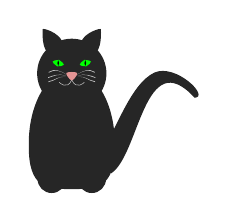
\begin{tikzpicture}
 \cat[eye=green]
\end{tikzpicture}}&
\scsnowman[scale=5,eyes, mouth,
nose, arms, hat=NavyBlue, muffler=Maroon,
buttons, snow, broom]&
\scalebox{6}{\twemoji{sushi}}&
\scalebox{6}{\twemoji{lemon}}\\
(a)&(b)&(c)&(d)
\end{tabular}
\bigskip

\Huge

\onslide<2->{a}%
\onslide<3->{n}%
\onslide<4->{i}%
\onslide<5->{m}%
\onslide<6->{a}%
\onslide<7->{l}%

\large
\mbox{}\hfill\visible<1->{\myaudio{./audio/quiz/answer_a.mp3}}

\end{frame}
%%%%%%%%%%%%%%%%%%%%%%%%%%%%
\begin{frame}<1,5>[plain]{Quiz}
 \large
\visible<1->{%
これからアルファベットを4つ順番に読みあげます。
聞こえたアルファベットを順番に小文字で書いてください。すると、ある単語になります。その意味を表す図を選んでください
}
\mbox{}\hfill\visible<1->{\myaudio{./audio/quiz/quiz_b.mp3}}

\bigskip

\centering
\begin{tabular}{c@{   }c@{   }c@{   }c}
\fcBike{.7}{Maroon}{1}&
\scalebox{6}{\twemoji{doughnut}}&
\scalebox{6}{\twemoji{sunflower}}&
\scalebox{6}{\twemoji{book}}\\
(a)&(b)&(c)&(d)
\end{tabular}

\bigskip

\Huge

\onslide<2->{b}%
\onslide<3->{o}%
\onslide<4->{o}%
\onslide<5->{k}%

\large
\mbox{}\hfill\visible<1->{\myaudio{./audio/quiz/answer_b.mp3}}


\end{frame}
%%%%%%%%%%%%%%%%%%%%%%%%%%%
%%%%%%%%%%%%%%%%%%%%%%%%%%%%%%%%%%%%%%%
\begin{frame}<1,6>[plain]{Quiz}
 \large
\visible<1->{%
これからアルファベットを5つ順番に読みあげます。
聞こえたアルファベットを順番に小文字で書いてください。すると、ある単語になります。その意味を表す図を選んでください
}
\mbox{}\hfill\visible<1->{\myaudio{./audio/quiz/quiz_c.mp3}}

\bigskip

\centering
\begin{tabular}{c@{   }c@{   }c@{   }c}
\scalebox{7}{\twemoji{carrot}}&
\scalebox{7}{\twemoji{doughnut}}&
\scalebox{7}{\twemoji{candy}}&
\scalebox{7}{\twemoji{cake}}\\
(a)&(b)&(c)&(d)
\end{tabular}

\bigskip

\Huge

\onslide<2->{c}%
\onslide<3->{a}%
\onslide<4->{n}%
\onslide<5->{d}%
\onslide<6->{y}%

\large
\mbox{}\hfill\visible<1->{\myaudio{./audio/quiz/answer_c.mp3}}
\end{frame}
%%%%%%%%%%%%%%%%%%%%%%%%%%%%%%%%%%%%%%%%%%%%%%%%%%
%\begin{frame}[plain]{candy}
%
%\includegraphics[height=.875\textheight]{./images/candy.jpg}
%
%\raggedleft
%\tiny
%"Lollipop 091" by greenbes is licensed under CC BY 2.0.\\
%To view a copy of this license, visit \url{https://creativecommons.org/licenses/by/2.0/?ref=openverse}.
%
%
% \end{frame}
%%%%%%%%%%%%%%%%%%%%%%%%%%%%
\begin{frame}<1,8>[plain]{Quiz}
 \large
\visible<1->{%
これからアルファベットを7つ順番に読みあげます。
聞こえたアルファベットを順番に小文字で書いてください。すると、ある単語になります。その意味を表す図を選んでください
}
\mbox{}\hfill\visible<1->{\myaudio{./audio/quiz/quiz_d.mp3}}

\bigskip

\centering
\begin{tabular}{c@{   }c@{   }c@{   }c}
\scalebox{7}{\twemoji{club suit}}&
\scalebox{7}{\twemoji{diamond suit}}&
\scalebox{7}{\twemoji{heart suit}}&
\scalebox{7}{\twemoji{spade suit}}\\
(a)&(b)&(c)&(d)
\end{tabular}

\bigskip
\Huge

\onslide<2->{d}%
\onslide<3->{i}%
\onslide<4->{a}%
\onslide<5->{m}%
\onslide<6->{o}%
\onslide<7->{n}%
\onslide<8->{d}

\large
\mbox{}\hfill\visible<1->{\myaudio{./audio/quiz/answer_d.mp3}}

\end{frame}
%%%%%%%%%%%%%%%%%%%%%%%%%%%%%%%%%%%%%%%%%%%%%%%%%%
%\begin{frame}[plain]{もちろん、これもdiamondです}
%
%\raggedleft
%
%\includegraphics[height=.95\textheight]{./images/diamonds.jpg}
%
%\vspace*{-8pt}
%\tiny
%
%Photo by \href{https://unsplash.com/@edgardo1987?utm_content=creditCopyText&utm_medium=referral&utm_source=unsplash}{Edgar Soto} on \href{https://unsplash.com/photos/two-diamond-studded-silver-rings-gb0BZGae1Nk}{Unsplash}
%\end{frame}
%%%%%%%%%%%%%%%%%%%%%%%%%%%%%%%%%%%%%%%%%%%%%%%%%%
\begin{frame}<1,6>[plain]{Quiz}
 \large
\visible<1->{%
これからアルファベットを5つ順番に読みあげます。
聞こえたアルファベットを順番に小文字で書いてください。すると、ある単語になります。
その意味を表すものを選んでください
}
\mbox{}\hfill\visible<1->{\myaudio{./audio/quiz/quiz_e.mp3}}

\bigskip

\centering
\begin{tabular}{c@{   }c@{   }c@{   }c}
\scalebox{2.236}{\epsdice{4}}\,\,\raisebox{5pt}{\LARGE $+$}\,\,\scalebox{2.236}{\epsdice{6}}&
\fcNumberNine{.1732}{NavyBlue}{1}&
{\Huge $3\times{}3-1$}&
\usymW{1F0C7}{1cm}

\\
(a)&(b)&(c)&(d)
\end{tabular}

\bigskip
\Huge

\onslide<2->{e}%
\onslide<3->{i}%
\onslide<4->{g}%
\onslide<5->{h}%
\onslide<6->{t}%

\large
\mbox{}\hfill\visible<1->{\myaudio{./audio/quiz/answer_e.mp3}}

\end{frame}
%%%%%%%%%%%%%%%%%%%%%%%%%%%%%%%%%%%%%%%%%%%%%%%%%%
\begin{frame}<1,5>[plain]{Quiz}
 \large
\visible<1->{%
これからアルファベットを4つ順番に読みあげます。
聞こえたアルファベットを順番に小文字で書いてください。すると、ある単語になります。
その意味を表すものを選んでください
}
\mbox{}\hfill\visible<1->{\myaudio{./audio/quiz/quiz_e.mp3}}

\bigskip

\centering
\begin{tabular}{c@{   }c@{   }c@{   }c}
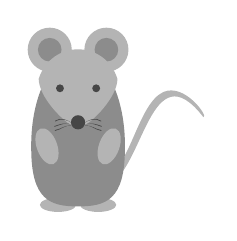
\begin{tikzpicture}
\mouse
\end{tikzpicture}&
\fcFishD{.15}{NavyBlue}{2}&
\scalebox{2}{\usymH{2614}{1cm}}&

\begin{tikzpicture}
\penguin
\end{tikzpicture}
\\
(a)&(b)&(c)&(d)
\end{tabular}

\bigskip
\Huge

\onslide<2->{f}%
\onslide<3->{i}%
\onslide<4->{s}%
\onslide<5->{h}%

\large
\mbox{}\hfill\visible<1->{\myaudio{./audio/quiz/answer_e.mp3}}

\end{frame}
%%%%%%%%%%%%%%%%%%%%%%%%%%%%%%%%%%%%%%%%%%%%%%%%%%
\begin{frame}<1,6>[plain]{Quiz}
 \large
\visible<1->{%
これからアルファベットを5つ順番に読みあげます。
聞こえたアルファベットを順番に小文字で書いてください。すると、ある単語になります。
その意味を表すものを選んでください
}
\mbox{}\hfill\visible<1->{\myaudio{./audio/quiz/quiz_e.mp3}}

\bigskip

\centering
\begin{tabular}{c@{   }c@{   }c@{   }c}
\scalebox{.8}{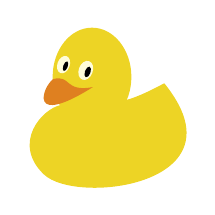
\begin{tikzpicture}
\duck
\end{tikzpicture}}&
\fcGhost{.67}{NavyBlue}{2}&
\raisebox{8pt}{\scalebox{4}{$\mathwitch$}}&
\raisebox{15pt}{\scalebox{3}{\Bigassumption}}
\\
(a)&(b)&(c)&(d)
\end{tabular}

\bigskip
\Huge

\onslide<2->{g}%
\onslide<3->{h}%
\onslide<4->{o}%
\onslide<5->{s}%
\onslide<6->{t}%

\large
\mbox{}\hfill\visible<1->{\myaudio{./audio/quiz/answer_e.mp3}}

\end{frame}
\end{document}
